\chapter{Per Video Rating}\label{cha:appendix-video-rating}
In this appendix, you will find an alternative way of studying the results from the subjective and the objective rating where each video with it's results has been plotted along the x-axis.

\begin{figure}[H]
    \centering
    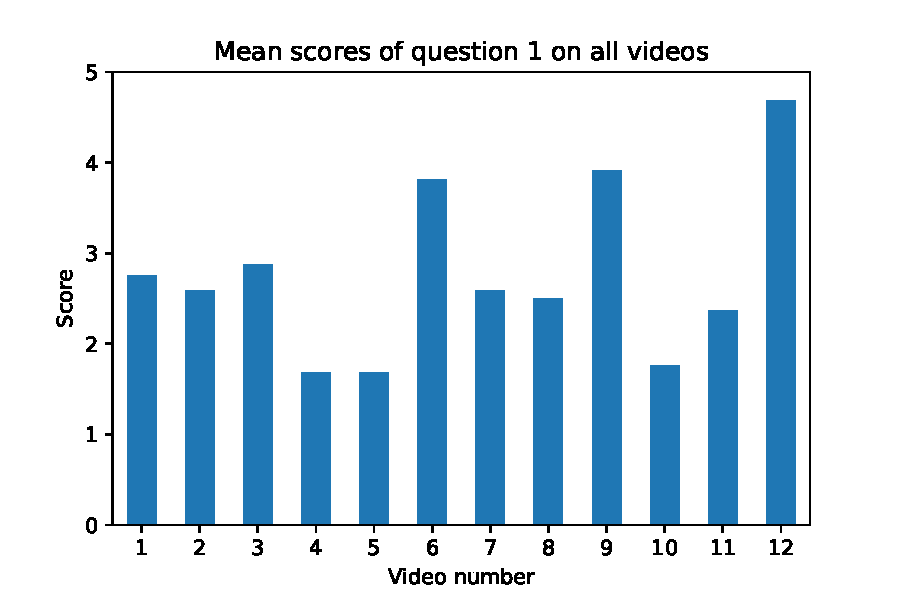
\includegraphics[width=0.8\textwidth]{img/questions/question_1.pdf}
    \caption{Average rating of question 1, ''How satisfied are you with the quality of the silhouette extraction?'', for all of the 12 videos.}
    \label{fig:video_rating_q1}
\end{figure}

\begin{figure}[H]
    \centering
    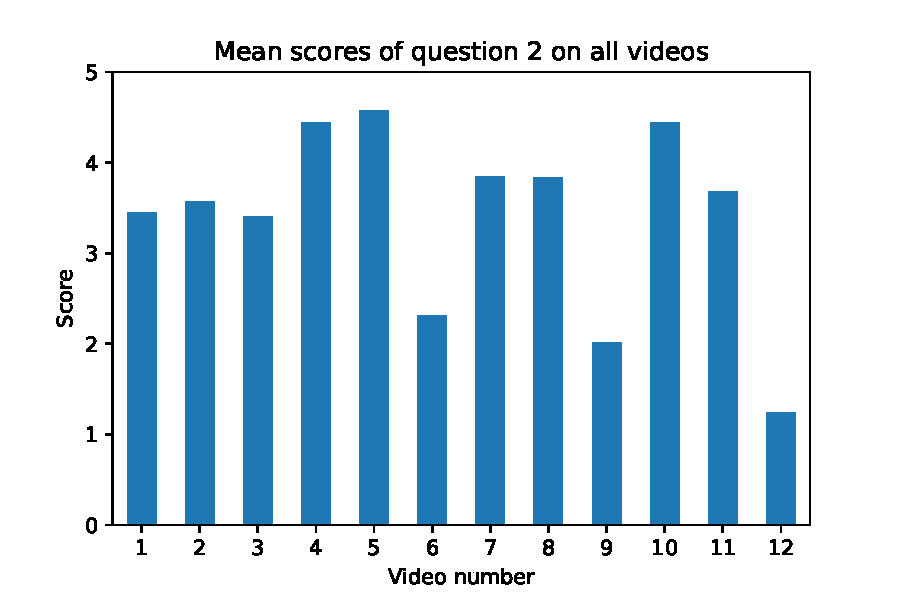
\includegraphics[width=0.8\textwidth]{img/questions/question_2.pdf}
    \caption{Average rating of question 2, ''Did you notice any artefacts with the silhouette extraction?'', for all of the 12 videos.}
    \label{fig:video_rating_q2}
\end{figure}


\begin{figure}[H]
    \centering
    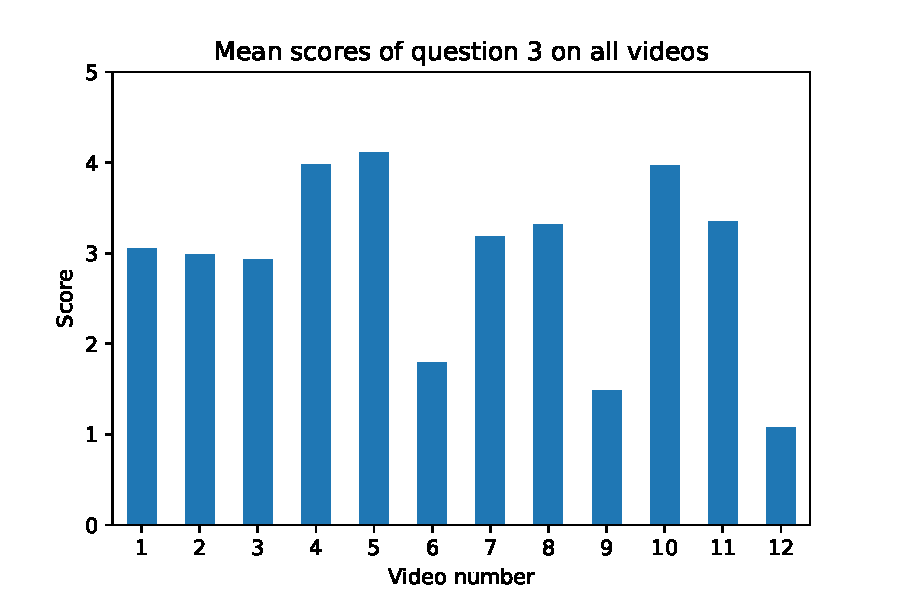
\includegraphics[width=0.8\textwidth]{img/questions/question_3.pdf}
    \caption{Average rating of question 3, ''Do you think the artefacts were annoying?'', for all of the 12 videos.}
    \label{fig:video_rating_q3}
\end{figure}


\begin{figure}[H]
    \centering
    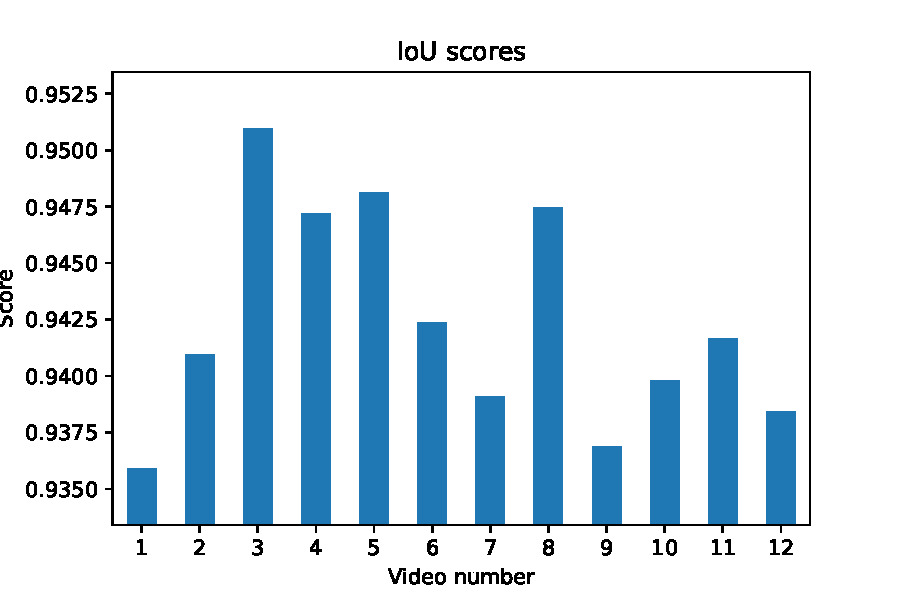
\includegraphics[width=0.8\textwidth]{img/results_objective_measures/IoU.pdf}
    \caption{Average rating of \acrlong{iou} for all of the 12 videos.}
    \label{fig:video_rating_iou}
\end{figure}

\begin{figure}[H]
    \centering
    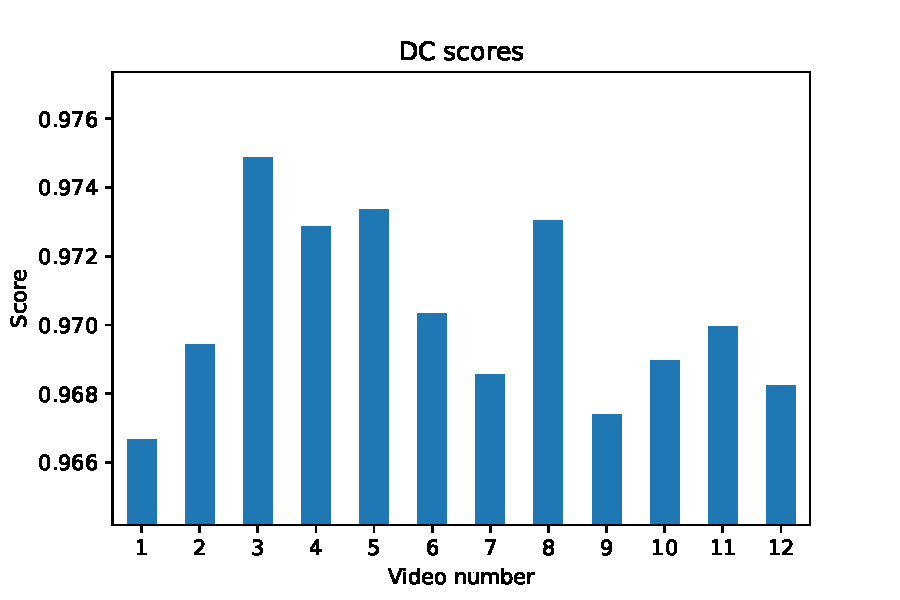
\includegraphics[width=0.8\textwidth]{img/results_objective_measures/DC.pdf}
    \caption{Average rating of \acrlong{dc} for all of the 12 videos.}
    \label{fig:video_rating_dc}
\end{figure}


\begin{figure}[H]
    \centering
    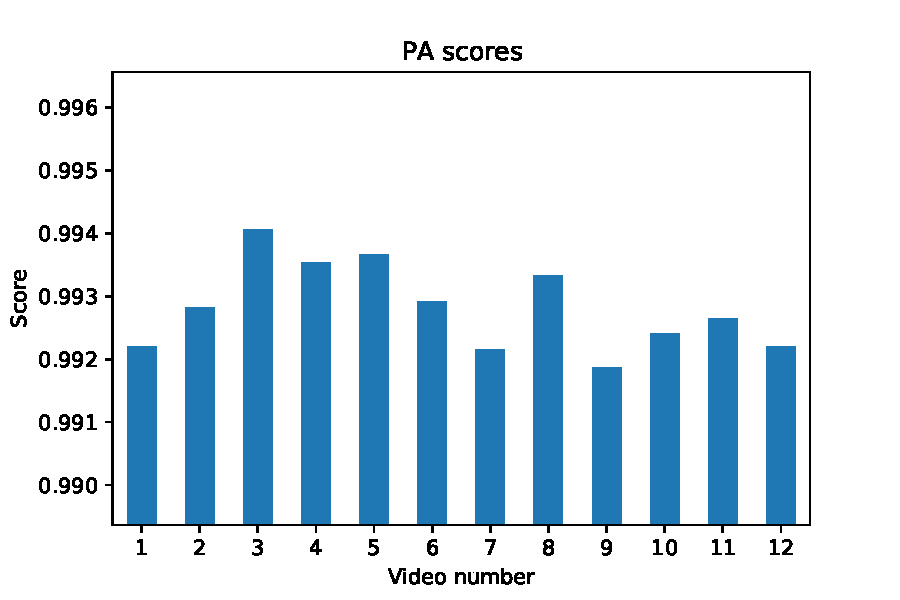
\includegraphics[width=0.8\textwidth]{img/results_objective_measures/PA.pdf}
    \caption{Average rating of \acrlong{pa} for all of the 12 videos.}
    \label{fig:video_rating_pa}
\end{figure}